\documentclass[aspectratio=169]{beamer}
\usepackage{graphicx} % Required for inserting images
\usepackage{listings}

\usepackage{xcolor}

\definecolor{codestring}{HTML}{e87d3e}
\definecolor{codetext}{HTML}{2e2e2e}
\definecolor{codecomment}{HTML}{797979}
\definecolor{codeoperands}{HTML}{6c99bb}
\definecolor{codekeywords}{HTML}{b05279}
\definecolor{codenumbers}{HTML}{9e86c8}

\lstset{
    language=[Sharp]C,
    columns=fullflexible
    rulecolor=\color{codecomment},
    commentstyle=\color{codecomment}\itshape,
    keywordstyle=\color{codekeywords},
    numberstyle=\tiny\color{codecomment},
    stringstyle=\color{codestring},
    basicstyle=\color{codetext}\ttfamily\scriptsize,
    classoffset=1, % starting new class
    otherkeywords={>,<,;,=,~,!=,?,:,&&,||},
    morekeywords={>,<,;,=,~,!=,?,:,&&,||},
    keywordstyle=\color{codeoperands},
    literate=*
        {false}{{{\color{codenumbers}false}}}{5}
        {true}{{{\color{codenumbers}true}}}{4}
        {0}{{{\color{codenumbers}0}}}{1}
        {1}{{{\color{codenumbers}1}}}{1}
        {2}{{{\color{codenumbers}2}}}{1}
        {3}{{{\color{codenumbers}3}}}{1}
        {4}{{{\color{codenumbers}4}}}{1}
        {5}{{{\color{codenumbers}5}}}{1}
        {6}{{{\color{codenumbers}6}}}{1}
        {7}{{{\color{codenumbers}7}}}{1}
        {8}{{{\color{codenumbers}8}}}{1}
        {9}{{{\color{codenumbers}9}}}{1}
        {.}{{{\color{codenumbers}.}}}{1}
        {0f}{{{\color{codenumbers}0f}}}{2}
        {1f}{{{\color{codenumbers}1f}}}{2}
        {2f}{{{\color{codenumbers}2f}}}{2}
        {3f}{{{\color{codenumbers}3f}}}{2}
        {4f}{{{\color{codenumbers}4f}}}{2}
        {5f}{{{\color{codenumbers}5f}}}{2}
        {6f}{{{\color{codenumbers}6f}}}{2}
        {7f}{{{\color{codenumbers}7f}}}{2}
        {8f}{{{\color{codenumbers}8f}}}{2}
        {9f}{{{\color{codenumbers}9f}}}{2},
    classoffset=0,
    breakatwhitespace=false,
    breaklines=true,         
    captionpos=b,   
    keepspaces=false,
    showspaces=false,
    showstringspaces=false,
    showtabs=false,
    tabsize=2
}
\lstnewenvironment{codeblock}
{\hfill\lstset{frame=single}\minipage{\textwidth}}
{\endminipage\hfill\null}

\usetheme{b2b}

\title{Back To Debug}
\author{Julie Fiadino}
\date{November 2023}

\begin{document}

%\newenvironment{infobox}[2]
%{
%\begin{tcolorbox}[enhanced,title=#1, frame style tile={width=\paperwidth}{img/b2b_bg.png}]
%#2}
%{\end{tcolobox}}

\maketitle

\section{Le guide du parfait SUP}

\begin{frame}{Frame}

\begin{enumerate}
    \item<1-7> Lire le sujet
    \item<2-7> \textbf<2>{Bien lire le sujet} (j'insiste)
    \item<3-7> Réfléchir à comment écrire la fonction
    \item<4-7> Relire le sujet
    \item<5-7> Coder sa fonction
    \item<6-7> Faire des Unit tests
    \item<7- | alert @8> Debugger les cas où ça ne marche pas
\end{enumerate}
\end{frame}

\section{Debugger c'est quoi ?}

\subsection{Les exemples à ne pas faire}

\begin{frame}{Frame}
    Debugger, ce n'est pas :

    \begin{enumerate}
        \item<2-> Regarder son code pendant 20min
        \item<3-> Retirer les tests qui ne marchent pas
    \end{enumerate}
\end{frame}

\subsection{Debugger avec Rider}
\begin{frame}{Frame Title}    
\begin{figure}
    \centering
    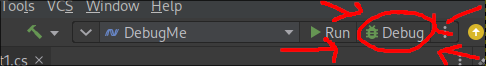
\includegraphics[width=\textwidth]{img/bouton_debug.png}
    \caption{Le bouton Debug}
    \label{fig:debug-button}
\end{figure}
\end{frame}

\begin{frame}{Frame Title}
\begin{figure}
    \centering
    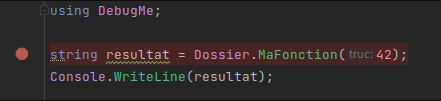
\includegraphics[width=\textwidth]{img/breakpoint.png}
    \caption{Ajouter un breakpoint}
    \label{fig:breakpoint}
\end{figure}
\end{frame}

\begin{frame}{Frame Title}
\begin{figure}
    \centering
    
\includegraphics[width=\textwidth]{img/debug_bar.png}
    \caption{Les outils du Debug}
    \label{fig:debug-bar}
\end{figure}
\end{frame}

\section{Quelques exemples}
\subsection{Dessiner des losanges}

\begin{frame}[fragile]
\frametitle{Frame Title}
    Écrire une fonction qui renvoie une string formant un losange de taille
    $2n + 1$, dessiné avec le caractère $c$.\\
    Une fois que le nombre requis de caractère $c$ a été écrit, il faut ajouter
    immédiatement un \textbackslash n.\\
    Si $n < 0$, renvoyer une string vide.\\~\

    \begin{infobox}{Prototype}
    \begin{lstlisting}
public static string Losange(char c, int n) { }
    \end{lstlisting}
    \end{infobox}
\end{frame}

\begin{frame}[fragile]
\frametitle{Truc}
    \begin{infobox}{Exemple}
    \begin{lstlisting}
string l1 = Losange(`*', 1); // == " *\n***\n *\n"
string l2 = Losange(`_', 2); // == "  _\n ___\n_____\n ___\n  _\n"
Console.WriteLine(l1);
Console.WriteLine(l2);
    \end{lstlisting}
    \end{infobox}
\end{frame}

\begin{frame}[fragile]
\frametitle{Truc}
    \begin{infobox}{Output}
    \begin{lstlisting}
 * 
***
 * 
 
  _  
 ___ 
_____
 ___
  _
    \end{lstlisting}
    \end{infobox}
\end{frame}

\section{Debugger - Le retour}
\subsection{Avec des Unit tests}

\begin{frame}{Frame Title}    
\begin{figure}
    \centering
    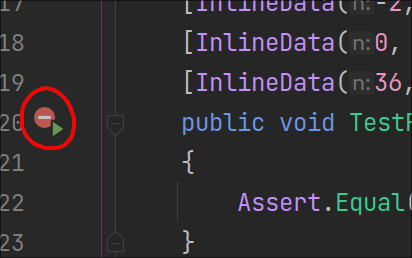
\includegraphics[height=6cm]{img/debug_unit.png}
    \caption{Debugger via son code}
    \label{fig:debug-button}
\end{figure}
\end{frame}

\begin{frame}{Frame Title}    
\begin{figure}
    \centering
    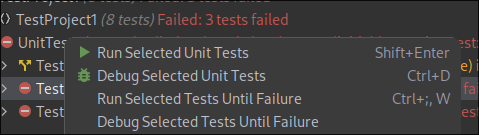
\includegraphics[width=\textwidth]{img/debug_unit_panel.png}
    \caption{Relancer un unit test}
    \label{fig:debug-button}
\end{figure}
\end{frame}

\section{Toujours plus d'exemples}
\subsection{Des erreurs chez les minuscules}

\begin{frame}{Frame Title}
    Schtroumpf Codeur a écrit une fonction qui lui indique si une string est
    composée uniquement de caractères en minuscule.\\
    \pause
    Mais sa fonction lève une erreur quand le test est valide.
\end{frame}

\subsection{Des nombres et des nombres et des nombres}

\begin{frame}{Frame Title}
    Schtroumpf Ingénieur a besoin de calculer la somme des puissances de 3 pour
    sa nouvelle invention.\\
    \pause
    Le problème, c'est que sa fonction ne renvoie pas toujours les valeurs
    attendues.
\end{frame}

\subsection{Un peu de récursion}

\begin{frame}{Frame Title}
    Schtroumpf à Lunettes s'est essayé aux joies de la récursion. Il a décidé de
    concevoir un programme qui calcule la puissance d'un nombre de manière bien
    plus optimisée qu'une boucle classique.\\
    \pause
    Mais pour lui non plus, le programme ne marche pas.
\end{frame}

\end{document}
